%===============================================================================
\chapter{Identifica��o de sistemas lineares invariantes no tempo de tempo discreto}
\label{chapter:system_identification}
%===============================================================================

Neste capitulo ser� abordada uma breve introdu��o e apresenta��o sobre identifica��o de sistemas
lineares. Inicialmente ser� apresentado uma introdu��o com alguns dos principais fatos que motivam
a utiliza��o de identifica��o de sistemas (Se��o \ref{sec:sys_ident_objective}).

Em seguida ser� apresentado algumas das principais caracter�sticas e o que comp�em a identifica��o de 
sistemas. Ser� descrito as principais caracter�sticas e atribui��es do conjunto de dados 
utilizado para a identifica��o (Se��o \ref{sec:sys_ident_data_acquisition}) e algumas das caracter�sticas e 
utiliza��es de projetos de experimentos (Se��o \ref{sec:si_project_experiments}).

Na Se��o \ref{sec:sys_ident_modelling_choosing} ser� apresentado de forma sucinta algumas classes
mais comumente utilizadas para a modelagem de sistemas lineares. Em seguida ser�o apresentado algumas
caracter�sticas pertinentes a identifica��o de sistemas com rela��o a propriedades das estimativas obtidas 
(Se��o \ref{sec:sys_ident_parameters_estimation}).

Ao fim ser� apresentado uma breve conclus�o sobre o que foi apresentado neste cap�tulo.

%===============================================================================
% Chapters
%===============================================================================
%===============================================================================
\section{Objetivo}
\label{sec:sys_ident_objective}
%===============================================================================

Identifica��o de sistemas possui uma vasta aplicabilidade em in�meros ramos do conhecimento,
n�o � escopo deste trabalho enumerar todas as possibilidades de utiliza��o desta ferramenta, nem t�o pouco 
esmiu�ar sua teoria. Ser�o aqui abordadas as principais caracter�sticas e princ�pios que comp�em a teoria de 
identifica��o de sistemas lineares.

O principal objetivo da identifica��o de um sistema � encontrar um modelo matem�tico que melhor consiga
descrever o sistema real sob observa��o, nas caracter�sticas desejadas escolhidas.

Pode-se considerar $y(t)$ como a sa�da do modelo matem�tico quando submetido a uma entrada $u(t)$ e
$\hat{y}(t)$ a sa�da real do sistema quando excitado pelo sinal de entrada $u(t)$. Os sinais $u(t)$
e $\hat{y}(t)$ s�o medidos pelo usu�rio.

Considerando o erro entre o sinal real $\hat{y}(t)$  e o sinal do modelo matem�tico $y(t)$ como:

\begin{equation}
\varepsilon (t)=y(t)-\hat{y}(t)
\nonumber
\end{equation}

A regress�o linear � o tipo mais simples de modelo param�trico. A estrutura do modelo
pode ser descrita como abaixo. \cite{system_identification}

\begin{equation}
\hat{y}(t)=\varphi ^T(t)\theta
\label{eq:si_obj_single_var}
\end{equation}

Onde $y(t)$ � chamada de {\it{vari�vel regredida}} e � medida do processo.
$\varphi (t)$ � comumente chamado de {\it{vari�vel de regress�o}} e $\theta$ � o vetor de
par�metros a ser identificado.

Assim, o erro pode ser reescrito como:

\begin{equation}
\varepsilon (t)=\hat{y}(t)-\varphi ^T(t)\theta
\nonumber
\end{equation} 

O objetivo da identifica��o de sistema, pode ser ent�o expresso como a escolha de um vetor $\hat{\theta}$ que
minimize a fun��o custo:

\begin{equation}
V(\theta)=\frac{1}{2}\sum_{t=1}^{N}\varepsilon ^2(t)=\frac{1}{2}\varepsilon^T\varepsilon=\frac{1}{2}\left \| \varepsilon \right \|
\label{eq:si_obj_etim_lsm_v}
\end{equation}

Com a minimiza��o do erro $\varepsilon (t)$ encontra-se um conjunto de parametros $\theta$ que melhor
consegue representar o relacionamento entre os sinais de entrada $u(t)$ e de sa�da $\hat{y}(t)$. 

%===============================================================================
\subsection{Identificabilidade de sistemas}
\label{sec:si_par_estim_sys_ident}
%===============================================================================

A identificabilidade de um sistema pode ser definido pelo teorema (\ref{theorem:identificability}).

\begin{theorem} 
\cite{ljung}

Considerando a estrutura de modelo $\mathcal{M}$ correspondente a: 
\begin{equation}
A(q)y(t)=\frac{B(q)}{F(q)}u(t)+\frac{C(q)}{D(q)}e(t)
\label{eq:si_par_estim_sys_theorem}
\end{equation}

e com $\theta$ sendo o coeficiente dos polin�mios envolvidos. Os graus dos polin�mios s�o $n_a$, $n_b$ e
assim por diante. A estrutura deste modelo � globalmente identific�vel se, e somente se, todos os itens de
(i) at� (vi) forem verdadeiros.

\begin{enumerate}[(i)]
\item N�o existe fator comum para todos os $z^{na}A^*(z), z^{nb}B^*(z), and, \; z^{nc}C^*(z)$.
\item N�o existe fator comum para $z^{nb}B^*(z), and, \; z^{nf}F^*(z)$.
\item N�o existe fator comum para $z^{nc}C^*(z), and, \; z^{nd}D^*(z)$.
\item Se $n_a \geq 1$ ent�o n�o pode existir fator comum entre $z^{nf}F^*(z), and, \; z^{nd}D^*(z)$.
\item Se $n_d \geq 1$ ent�o n�o pode existir fator comum entre $z^{na}A^*(z), and, \; z^{nb}B^*(z)$.
\item Se $n_f \geq 1$ ent�o n�o pode existir fator comum entre $z^{na}A^*(z), and, \; z^{nc}C^*(z)$.
\end{enumerate}

Os polin�mios com $*$ correspondem a $\theta^*$
\label{theorem:identificability}
\end{theorem}

Note que as condi��es de (i) at� (vi) s�o satisfeitas para o caso comum de \eqref{eq:si_par_estim_sys_theorem}.
Observe tamb�m que nenhuma das condi��es pode ser violada por qualquer {\it{especial}} valor de $\theta^*$, posto na
hiper-superf�cie de $\Re ^d$. Isso nos leva ao seguinte corol�rio:

\begin{cor} 
A estrutura de modelo apresentada em \eqref{eq:si_par_estim_sys_theorem} � globalmente identific�vel.
\label{corollary:identificability}
\end{cor} 

A partir do Corol�rio (\ref{corollary:identificability}) temos que a identifica��o de sistemas
utilizando os fam�lias ou conjuntos de modelos descritos por \eqref{eq:si_par_estim_sys_theorem}
s�o globalmente identific�veis se tivermos dados de entrada suficientemente informativos.


%===============================================================================
\section{Conjunto de dados coletados}
\label{sec:sys_ident_data_acquisition}
%===============================================================================

Identifica��o de sistemas � baseada no conjunto de dados coletados do sistema
observado. Estes dados podem ser obtidos em regime normal de opera��o ou sob
condi��es pr� determinadas, onde � poss�vel escolher previamente o sinal de
entrada que ser� aplicado sobre o sistema. Isso � feito para que os dados
coletados sejam o mais informativos poss�veis. \cite{ljung} Maiores detalhes
sobre escolha de sinais para alimenta��o ser�o abordados no capitulo sobre 
projeto de experimentos (se��o (\ref{sec:si_project_experiments})).




%===============================================================================
\subsection{Considera��es em modelagem}
\label{sec:sys_ident_basic_definitions}
%===============================================================================

Geralmente, na modelagem de sistemas algumas considera��es s�o feitas sobre o este:

{\it{Linearidade}}. Uma considera��o frequentemente feita � a de se supor que o sistema sendo modelado se
comporta de forma aproximadamente linear. Tal suposi��o � normalmente verificada observando-se o comportamento
em uma faixa relativamente estreita de opera��es. \cite{aguirre}

Formalmente diz-se que um sistema � linear se ele obedece o {\it{princ�pio da superposi��o}}.  A considera��o
da linearidade normalmente simplifica bastante o modelo a ser constru�do.
Entretanto, h� situa��es em que esta considera��o n�o � adequada, como por exemplo, para sistemas como
din�mica fortemente bilinear (que n�o podem ser descritos adequadamente por um �nico modelo linear,
independentemente de qu�o estreita seja a faixa de opera��o considerada). E tamb�m no caso onde se deseja
estudar caracter�sticas din�micas n�o-lineares do sistema, tais como oscila��es e bifurca��es.  \cite{aguirre}

{\it{Invari�ncia no tempo}}. A considera��o de invari�ncia temporal implica que o comportamento do sistema
sendo identificado n�o varia com o tempo. Formalmente diz-se que um sistema � invariante se um deslocamento no
tempo na entrada causa um deslocamento no tempo na sa�da.



%===============================================================================
\section{Estimativa de par�metros}
\label{sec:sys_ident_parameters_estimation}
%===============================================================================

A estimativa dos par�metros dos modelos dependem de v�rios fatores. At� agora foi apresentado
a import�ncia dos dados coletados (Se��o (\ref{sec:sys_ident_data_acquisition})) e da 
escolha do modelo (Se��o (\ref{sec:sys_ident_modelling_choosing})). Nesta se��o ser�o 
apresentadas algumas formas para a estimativa dos par�metros, bem como algumas de suas
caracter�sticas probabil�sticas. 

A identifica��o � baseada em um conjunto de dados coletados do sistema, um modelo para caracteriz�-lo.
Um preditor � uma equa��o que tenta prever o pr�ximo valor do sistema baseado nos dados passados deste.
Com o preditor atinge-se um conjunto de dados que deve ser muito pr�ximo aos dados verdadeiros
coletados do sistema. Escolhe-se ent�o um m�todo para minimiza��o do erro existente entre
os dados coletados e os dados calculados pelo preditor.

Por fim ser�o apresentados algumas das caracter�sticas para a estima��o quando alguns 
requisitos para a identifica��o n�o s�o atingidos, como por exemplo quando o modelo
escolhido n�o consegue representar o sistema, ou quando o dados de entrada n�o s�o 
suficientemente informativos. Nestas situa��es teremos erros na estimativa dos par�metros.
Erros diferentes que ser�o abordados na se��o (\ref{sec:si_par_estim_uncertanties}).






%===============================================================================
\section{Projeto de Experimento}
\label{sec:si_project_experiments}
%===============================================================================

Projeto de experimentos pode ser entendido como o procedimento para que se escolha o melhor 
sinal de entrada para a identifica��o dos par�metros desejados para o experimento. 
Desta forma muitas vari�veis podem ser levadas em considera��o, refletindo em propriedades que
podem ou n�o ser o foco do projeto de experimentos.

Uma forma de organizar o projeto de experimento � desenvolve-lo como um problema de otimiza��o 
convexa, onde entre muitas vantagens est� o fato de que � poss�vel a utiliza��o de m�todos matem�ticos
para o seu c�lculo e sua formula��o pode ser feita por LMI ({\it{Linear Matrix Inequality}}. Em \cite{jansson}
este t�pico � explorado em mais profundidade, sendo aqui apenas apresentado a sua ideia b�sica.
Este t�pico � abordado na se��o (\ref{sec:si_project_optimization}).

O projeto de experimento � uma alternativa ao uso de sinais como PRBS ({\it{Pseudo Randon Binary Sequence}}).
A escolha de um sinal mais apropriado para o experimento traz diversas vantagens, que podem ser bastante
significativas para o tempo e esfor�o despendido sobre o projeto do controlador, ou da identifica��o do sistema.
Uma destas vantagens � o tempo de dados coletados, aplicando-se sinais com componentes de frequ�ncia que s�o
mais informativos, tem-se uma efici�ncia maior nos dados amostrados, bastando um montante menor de data, para que
sejam obtidos os mesmos �ndices de qualidade, quando comparado com projetos utilizando sinais mais simples.

%===============================================================================
\subsection{Sinais de entrada mais comumente utilizados}
\label{sec:si_project_signal_input}
%===============================================================================

Como foi apresentado no capitulo (\ref{sec:si_data_persistently_excitation}) �
poss�vel formar sinais persistentes, apenas adicionando um n�mero suficiente de componentes
de frequ�ncia a fim de que todos os par�metros possam ser estimados. N�o � estranho
que se pense que quanto mais componentes tiver o sinal, melhor. 

Desta maneira, v�rios sinais que podem ser gerados de maneira f�cil e que possuem 
um grande range de componentes de frequ�ncia foram elaborados.

%===============================================================================
\subsubsection{Sinal Bin�rio Rand�mico}
\label{sec:si_project_signal_input_rbs}
%===============================================================================

Um sinal bin�rio por defini��o assume apenas dois valores (0 ou 1). Partindo deste
principio, um sinal bin�rio rand�mico, � uma sequencia aleat�ria de zeros e uns, que
formam o sinal.

A forma mais simples para a gerar este sinal �, baseado em um ruido Gausiano branco
de m�dia zero, aplicar um filtro linear previamente escolhido. Assim pode-se teoricamente
gerar qualquer sinal bin�rio de qualquer n�vel.

O inconveniente desta forma � que aplicando um filtro ao sinal Gausiano ir� alterar o
seu espectro, n�o sendo a forma desta altera��o algo conhecido. Deve-se ent�o sempre 
antes de aplicar o sinal no sistema, verificar o espectro gerado. \cite{ljung}


%===============================================================================
\subsubsection{Sinal Bin�rio Pseudo-Rand�mico - PRBS}
\label{sec:si_project_signal_input_prbs}
%===============================================================================
% ref: ljung pages 418

Um {\it{sinal bin�rio pseudo-rand�mico}} � um sinal peri�dico com algumas propriedades
semelhantes a de ruido branco. Este sinal � gerado pela equa��o \eqref{eq:si_project_signal_prbs}.

\begin{equation}
u(t)=rem(A(q)u(t), 2)=rem(a_1 u(t-1)+...+a_n u(t-n), 2)
\label{eq:si_project_signal_prbs}
\end{equation}

Onde $rem(x, 2)$ � o resto inteiro da divis�o de $x$ por 2. O sinal $u(t)$ deve ser peri�dico 
de pelo menos $2^n$ valores diferentes, como uma sequencia de zeros n�o � um sinal v�lido, por ser nulo, 
temos que o m�ximo per�odo � de tamanho $M=2^n -1$. Na verdade o per�odo vai depender da
escolha de $A(q)$. Pode-se entretanto mostrar que para cada $n$ existem escolhas de $A(q)$ que 
proporcionam o tamanho m�ximo. Tais escolhas s�o apresentadas na Tabela (\ref{table:si_project_input_prbs}).
\cite{ljung}

\begin{table*}[htbp]
\begin{center}
\caption{Polin�mios $A(q)$ que geram o m�ximo per�odo $M$ para sinais PRBS de ordem $n$. $a_k=1$ para os $k$
   	indicados, 0 para os demais. Diversas outras escolhas existem para os mesmos $n$.}
\label{table:si_project_input_prbs}
\begin{tabular}{ccc}
\hline
        Ordem $n$ & $M=2^n-1$ & $a_k$ n�o zeros para $k$   \\
\hline
        2       & 3        & 1, 2       \\
        3       & 7        & 2, 3       \\
        4       & 15       & 1, 4       \\
        5       & 31       & 2, 5       \\
        6       & 63       & 1, 6       \\
        7       & 127      & 3, 7       \\
        8       & 255      & 1, 2, 7, 8 \\
        9       & 511      & 4, 9       \\
        10      & 1023     & 7, 10      \\
        11      & 2047     & 9, 11      \\
\hline
\end{tabular}
\end{center}
\end{table*}

O espectro de um sinal PRBS � dado por:

\begin{equation}
\Phi_u(\omega)=\frac{2 \pi \bar{u}^2}{M}\sum_{k=1}^{M-1}\delta (\omega -2 \pi k/M), \;\; 0\le \omega < 2 \pi
\label{eq:si_project_signal_prbs_spectrum}
\end{equation}

Observa-se que este � um sinal persistentemente excitante de ordem $M-1$. Na Figura 
(\ref{fig:si_project_prbs}) � apresentado um exemplo de sinal PRBS para $n=7$.

\begin{figure}[htbp]
	\center
	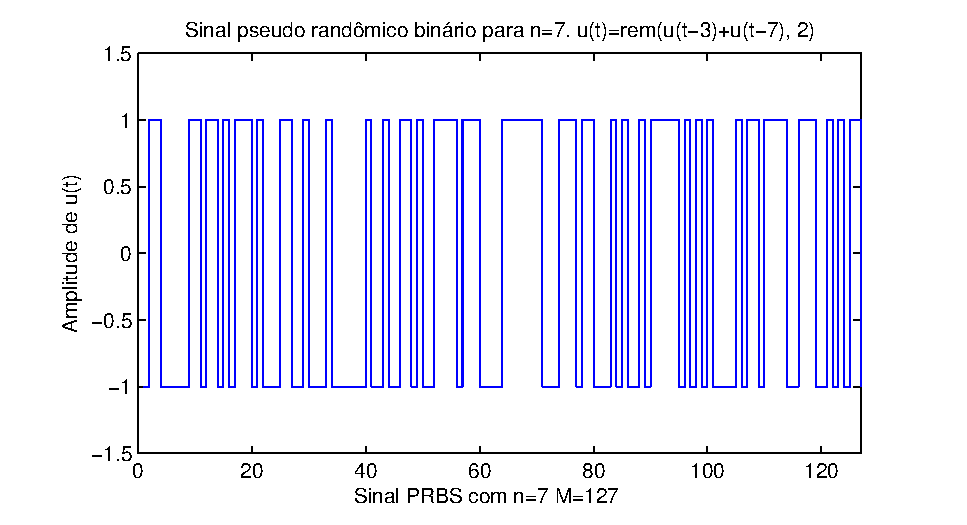
\includegraphics[width=0.95\columnwidth]{figures/si_project_prbs.eps}
	\caption{Sinal PRBS para $n=7$}
	\label{fig:si_project_prbs}
\end{figure}

As vantagens e desvantagens do sinal PRBS comparado com um ruido rand�mico bin�rio pode ser
listado: \cite{ljung}

\begin{enumerate}[(I)]
\item Se o PRBS possuir per�odos inteiros a sua matriz de covari�ncia ter� alguns padr�es bem espec�ficos que permitem 
analiticamente se fa�a uma invers�o desta matriz. Isso facilita certas computa��es.
\item Existem essencialmente apenas um PRBS para cada escolha de $A(q)$. Diferentes valores iniciais apenas deslocam a
sequencia.
\item Para que as propriedades vantajosas do PRBS possam ser utilizadas, � necess�rio que um numero inteiro de per�odos
seja utilizado, o que limita a escolha do tamanho do experimento.
\end{enumerate}

%===============================================================================
\subsubsection{Ruido Branco Filtrado}
\label{sec:si_project_signal_input_wn_filtered}
%===============================================================================

Um das escolhas mais simples de sinais, � gerar um ruido Gausiano e ent�o filtra-lo com 
algum filtro linear. Desta forma, teoricamente, � poss�vel de se atingir qualquer espectro de
sinal, bastando apenas a correta escolha do filtro. Como este sinal � gerado {\it{off-line}}, 
� poss�vel aplicar filtros n�o causais e eliminar efeitos transientes do sinal, o que
proporciona um comportamento espectral melhor. \cite{campestrini, ljung}

%===============================================================================
\subsection{Projeto de experimento como um problema de otimiza��o}
\label{sec:si_project_optimization}
%===============================================================================

O problema de projeto de experimento pode ser considerado como uma forma geral apresentada em \eqref{eq:si_project_optimization}

\begin{equation}
\begin{matrix}
\underset{\Phi_{\chi_0}}{\text{minimize}} &  & \text{Objetivo}\\ 
\text{Sujeito a:} &  & \text{Requisitos de qualidade}\\ 
 &  & \text{Requisitos de sinais}
\end{matrix}
\label{eq:si_project_optimization}
\end{equation}

De forma geral os requisitos de qualidades s�o fun��es da covari�ncia de $P$. Por esta raz�o � natural usar
o espectro da entrada $\Phi_u$ e eventualmente o espectro cruzado $\Phi_{ue}$ como vari�veis do projeto.
A inclus�o de limita��es nos sinais e sua inclus�o como vari�veis de projeto s�o �teis para evitar que se chegue
em resultados onde a energia de entrada precise ser infinita para se obter os crit�rios desejados, ou largura
de banda que n�o s�o facilmente ating�veis em projetos reais.

T�picos projetos de experimentos s�o intrat�veis em sua forma original, pelos seguintes motivos: \cite{jansson}

\begin{enumerate}[(I)]
\item Algumas restri��es s�o tipicamente n�o convexas, e problemas com estas caracter�sticas podem ser dif�ceis
de resolver.
\item Existem restri��es que s�o de dimens�o infinita, o que exigem um certo grau de cuidado no procedimento de
otimiza��o.
\item Existe ainda o problema de encontrar um sinal realiz�vel que tenha as propriedades desejadas para o espectro.
\item A vari�ncia assint�tica depende tipicamente dos par�metros do sistema $\theta_0$, $P=P(\theta_0)$ que s�o
desconhecidos.
\end{enumerate}

Os primeiros 3 itens listados acima s�o contorn�veis pela inser��o de uma parametriza��o finita do espectro de entrada
e algumas vezes at� do espectro cruzado, tornando o problema convexo, que pode ser tratado de forma bem mais f�cil.

O �ltimo item onde a solu��o do problema depende das caracter�sticas do sistema a ser identificado � intr�nseco de quase
todos os problemas de otimiza��o, sendo ent�o inevit�vel. Em problemas reais este fato pode ser contornado utilizando alguns
m�todos conhecidos. \cite{jansson}

A formula��o de um projeto de experimento pode ser particionado nas seguintes partes:

\renewcommand{\labelitemi}{$\bullet$}
\begin{itemize}

\item {\it{Parametriza��o do espectro}}

A escolha de usar uma parametriza��o finita do espectro ou uma parametriza��o parcial da correla��o � regido pelos seguintes
aspectos:

\begin{itemize}
\item relativos a otimiza��o
\item Computacionais
\item limita��o de sinais
\item robustez
\end{itemize}

A parametriza��o parcial da correla��o � �tima e pode usar um n�mero m�nimo de par�metros, utilizando assim, menos processamento
computacional. Entretanto certas limita��es de sinais n�o podem ser garantidas nesta situa��o, e a parametriza��o
pode depender do sistema real. Parametriza��o finita do espectro geralmente n�o atinge um m�nimo global mas as fun��es bases
n�o precisam ser fun��es do sistema real. Este m�todo pode gerenciar problemas de limita��es de sinal de frequ�ncia por frequ�ncia.
%-------------------------
\item {\it{Restri��es de qualidade}}

Assumindo que erros de vari�ncia s�o de grande import�ncia � natural que qualquer medida de qualidade do modelo leve em conta 
a matriz de covari�ncia $P$. Esta matriz pode ser manipulada pelos espectros de entrada $\Phi_{u}$ e o espectro cruzado $\Phi_{ue}$
como apresentado em \eqref{eq:si_project_optimization_quality}.

\begin{equation}
P^{-1}(\theta_0)=\frac{1}{2 \pi \lambda_0}\int_{-\pi}^{\pi}\mathcal{F}(e^{j\omega}, \theta_0)\begin{bmatrix}
\Phi_u(\omega) & \Phi_{ue}(\omega)\\ 
\Phi_{ue}^{*}(\omega) & \lambda_0 
\end{bmatrix}\mathcal{F}(e^{j\omega}, \theta_0)\;d\omega
\label{eq:si_project_optimization_quality}
\end{equation}

O principal desafio neste ponto � tornar as restri��es convexas em $P^{-1}$.

%-------------------------
\item {\it{Restri��es de sinal}}

Podem ser inclu�dos, restri��es de energia para os sinais de entrada e sa�da do sistema bem como restri��es no sinal dependentes da
frequ�ncia deste.
%-------------------------
\item {\it{Restri��es de robustez}}

A solu��o de boa parte dos problemas de otimiza��o recaem na necessidade de se conhecer o sistema real. Isso nem sempre � poss�vel 
e uma das formas de contornar este problema � substituir o sistema real por uma aproxima��o deste. Devido aos erros de estimativa deste
sistema, tem-se a necessidade de se utilizar m�todos que garantam robustez deste sistema, para que quando submetido ao sistema real, 
o projeto ainda seja v�lido.
%-------------------------
\end{itemize}



%===============================================================================
\section{Considera��es Finais}
\label{sec:si_conclusions}
%===============================================================================

Neste capitulo foram apresentados os principais aspectos de um projeto para identifica��o 
de sistemas. Partindo-se da escolha do sinal de excita��o para o experimento onde podemos 
determinar o que � de fundamental import�ncia para a identifica��o e focar os esfor�os para
reduzir ao m�ximo erros nestes aspectos.

Apresentou-se neste quesito de projeto de experimento, a ideia de tornar a escolha do sinal, um
problema de otimiza��o, onde as restri��es s�o as margens de qualidade que desejamos para as
propriedades assint�ticas da estimativa, limita��es de sinais que conseguimos produzir e margens de 
robustez.

Apresentou-se conceitos sobre a escolha do modelo que ser� utilizado para caracterizar o sistema
observado e as propriedades assint�ticas da estimativa para casos onde o sistema real $\mathcal{S}$ n�o
faz parte da fam�lia de modelos $\mathcal{M}$. Esta situa��o onde o sistema real n�o consegue ser
representado completamente pelo modelo adotado, faz com que erros de polariza��o e de vari�ncia 
recaiam sobre a estimativa atingida. Tamb�m foram apresentados os modelos mais comumente utilizados
para a identifica��o de sistemas lineares.

De posse dos dados coletados e da fam�lia de modelos que acredita-se conter o sistema real, � poss�vel, 
com a ajuda de preditores, determinar os par�metros do modelo que descrevem o comportamento do sistema
observado.

Elege-se ent�o uma fun��o dependente do erro entre os dados coletados e os dados gerados pelo preditor. 
Afim de que se tenha a melhor estimativa poss�vel, m�todos de minimiza��o s�o utilizados para que esta 
fun��o dependente do erro, seja minimizada. Obtendo-se assim a melhor estimativa poss�vel 
para aquele conjunto de dados, modelo e crit�rio de minimiza��o escolhidos.

� percept�vel que a identifica��o de um sistema � uma tarefa que depende de um grande conjunto
relativamente grande de de fatores. De um lado isso � extremamente interessante, pois temos liberdade
de escolha e a possibilidade de focar nosso projeto pontos que s�o mais interessantes, em detrimento
de outros que n�o s�o relevantes para o sistema em quest�o. Por outro lado temos um conjunto de
vari�veis que, se n�o compreendidas corretamente, podem tornar este processo algo oneroso e muitas
vezes at� ineficiente.



%===============================================================================


